% L’IA agentique au quotidien — REX OpenCode & bonnes pratiques
% Build: latexmk -xelatex main.tex      (slides)
%        latexmk -xelatex notes.tex     (slides + speaker notes on a second screen)
\documentclass[aspectratio=169,9pt,t]{beamer}
\ifdefined\withnotes\setbeameroption{show notes on second screen=right}\fi

\usepackage{fontspec}
\usepackage{xcolor}
\usepackage{tikz}
\usetikzlibrary{arrows.meta,calc,positioning,shadows,decorations.pathmorphing}
\usepackage{pgfplots}
\pgfplotsset{compat=1.18}
\usepackage{booktabs,array,tabularx,colortbl}

% ------------------------------------------------------------------ fonts
% IBM Plex ships with TeX Live (package plex); Archivo is bundled in fonts/ (SIL OFL 1.1)
\setsansfont{IBMPlexSans}[Extension=.otf,
  UprightFont=*-Regular, BoldFont=*-SemiBold, ItalicFont=*-Italic, BoldItalicFont=*-SemiBoldItalic]
\setmonofont{IBMPlexMono}[Extension=.otf, UprightFont=*-Regular, BoldFont=*-SemiBold, Scale=0.95]
\newfontfamily\headfont{Archivo}[Path=fonts/, Extension=.ttf,
  UprightFont=*-700, BoldFont=*-800, LetterSpace=-2.5]
\newfontfamily\labelfont{IBMPlexMono}[Extension=.otf, UprightFont=*-Medium, BoldFont=*-SemiBold, LetterSpace=10, Scale=0.95]
\renewcommand{\familydefault}{\sfdefault}
\hyphenpenalty=10000 \exhyphenpenalty=10000 % no English hyphenation in French text

% ------------------------------------------------------------------ colours
\definecolor{paper}{HTML}{EEF1F5}   % light slides
\definecolor{navy}{HTML}{0C1222}    % dark slides
\definecolor{navy2}{HTML}{141B2E}   % cards on dark
\definecolor{navyline}{HTML}{263150}
\definecolor{blue}{HTML}{2347E8}    % accent on light
\definecolor{peri}{HTML}{7F9CFF}    % accent on dark
\definecolor{lime}{HTML}{C8F24A}    % signal
\definecolor{ink}{HTML}{0B0B0B}
\definecolor{body}{HTML}{4A5263}
\definecolor{mute}{HTML}{6B7385}
\definecolor{cline}{HTML}{DCE2EB}
\definecolor{dmute}{HTML}{98A2BA}
\definecolor{codebg}{HTML}{0A0F1D}

% mode colours (set per slide by \light, \dark, \limeslide)
\colorlet{fgc}{ink}\colorlet{stripc}{blue}\colorlet{eyebg}{blue}\colorlet{eyefg}{white}
\colorlet{eyelab}{blue}\colorlet{footc}{mute}\colorlet{numc}{blue}\colorlet{hairc}{cline}
\newif\ifstrip \striptrue
\newcommand{\light}{\setbeamercolor{background canvas}{bg=paper}\colorlet{fgc}{ink}\colorlet{stripc}{blue}%
  \colorlet{eyebg}{blue}\colorlet{eyefg}{white}\colorlet{eyelab}{blue}\colorlet{footc}{mute}\colorlet{numc}{blue}%
  \colorlet{hairc}{cline}\striptrue\setbeamercolor{normal text}{fg=ink}}
\newcommand{\dark}{\setbeamercolor{background canvas}{bg=navy}\colorlet{fgc}{white}\colorlet{stripc}{lime}%
  \colorlet{eyebg}{lime}\colorlet{eyefg}{navy}\colorlet{eyelab}{peri}\colorlet{footc}{dmute}\colorlet{numc}{lime}%
  \colorlet{hairc}{navyline}\striptrue\setbeamercolor{normal text}{fg=white}}
\newcommand{\limeslide}{\setbeamercolor{background canvas}{bg=lime}\colorlet{fgc}{ink}\colorlet{stripc}{lime}%
  \colorlet{eyebg}{ink}\colorlet{eyefg}{white}\colorlet{eyelab}{ink}\colorlet{footc}{ink!70}\colorlet{numc}{ink}%
  \colorlet{hairc}{ink!25}\stripfalse\setbeamercolor{normal text}{fg=ink}}

% ------------------------------------------------------------------ theme
\setbeamertemplate{navigation symbols}{}
\setbeamersize{text margin left=1.05cm,text margin right=1.05cm}
\setbeamertemplate{background}{%
  \ifstrip\begin{tikzpicture}[remember picture,overlay]
    \fill[stripc] (current page.south west) rectangle ($(current page.north west)+(0.11,0)$);
  \end{tikzpicture}\fi}

% eyebrow: numbered box + mono label
\newcommand{\eyenum}{00}\newcommand{\eyelabel}{}
\newcommand{\kicker}[2]{\renewcommand{\eyenum}{#1}\renewcommand{\eyelabel}{#2}}
\newcommand{\eyebrow}{%
  \tikz[baseline=(b.base)]\node[fill=eyebg,text=eyefg,inner xsep=2.2pt,inner ysep=1.6pt,font=\labelfont\fontsize{5.6}{6}\selectfont\bfseries](b){\eyenum};%
  \hspace{4pt}{\labelfont\fontsize{5.6}{6}\selectfont\color{eyelab}\MakeUppercase{\eyelabel}}}

\setbeamertemplate{frametitle}{%
  \vspace{0.42cm}%
  \eyebrow\par\vspace{0.16cm}%
  {\headfont\fontsize{17}{19}\selectfont\color{fgc}\raggedright\insertframetitle\par}%
  \vspace{0.32cm}}

\setbeamertemplate{footline}{%
  \begin{tikzpicture}[remember picture,overlay]
    \draw[hairc,line width=0.4pt] ($(current page.south west)+(1.05,0.78)$) -- ($(current page.south east)+(-1.05,0.78)$);
    \node[anchor=base west,inner sep=0,text=footc,font=\labelfont\fontsize{4.8}{5}\selectfont]
      at ($(current page.south west)+(1.05,0.42)$) {REX OPENCODE · IA AGENTIQUE AU QUOTIDIEN};
    \node[anchor=base east,inner sep=0,text=numc,font=\labelfont\fontsize{5.2}{5}\selectfont\bfseries]
      at ($(current page.south east)+(-1.05,0.42)$) {\insertframenumber};
  \end{tikzpicture}}

% ------------------------------------------------------------------ building blocks
\tikzset{
  card/.style={fill=white,draw=cline,line width=0.4pt,inner sep=0pt,
    drop shadow={opacity=0.06,shadow xshift=0pt,shadow yshift=-0.7pt}},
  dcard/.style={fill=navy,draw=navy,line width=0.4pt,inner sep=0pt},
  ncard/.style={fill=navy2,draw=navyline,line width=0.4pt,inner sep=0pt},
  hcard/.style={fill=navy2,draw=lime,line width=0.6pt,inner sep=0pt},
  bcard/.style={fill=white,draw=blue,line width=0.7pt,inner sep=0pt,
    drop shadow={opacity=0.06,shadow xshift=0pt,shadow yshift=-0.7pt}},
  flow/.style={-{Latex[length=3pt,width=3pt]},blue,line width=0.9pt},
}
% \cardbox[style]{width}{height}{content}  — content top-aligned with 6pt padding
\newcommand{\cardbox}[4][card]{%
  \tikz[baseline=(c.north)]\node[#1,anchor=north,inner sep=6pt](c){\begin{minipage}[t][\dimexpr#3-12pt\relax][t]{\dimexpr#2-12pt\relax}\raggedright\leavevmode#4\end{minipage}};}
\newcommand{\ctag}[2][blue]{\leavevmode{\labelfont\fontsize{5.2}{6}\selectfont\color{#1}\MakeUppercase{#2}\par}\vspace{2.5pt}}
\newcommand{\ctitle}[2][ink]{\leavevmode{\fontsize{7.6}{9}\selectfont\bfseries\color{#1}#2\par}\vspace{2pt}}
\newcommand{\cbody}[2][body]{\leavevmode{\fontsize{6.2}{8}\selectfont\color{#1}#2\par}}
\newcommand{\code}[2][blue]{\leavevmode{\ttfamily\fontsize{6.2}{8}\selectfont\color{#1}#2}}
\newcommand{\arr}{\tikz[baseline=-0.6ex]\draw[flow](0,0)--(0.34,0);}
% pull quote with a coloured rule
\newcommand{\pull}[2][blue]{%
  \par\noindent\begin{tikzpicture}
    \node[inner sep=0pt,anchor=north west,text width=\dimexpr\linewidth-9pt\relax,align=left,font=\fontsize{8.2}{10.5}\selectfont\bfseries,text=fgc] (q) at (9pt,0) {#2};
    \fill[#1] ($(q.north west)+(-9pt,1.5pt)$) rectangle ($(q.south west)+(-7.8pt,-1.5pt)$);
  \end{tikzpicture}\par}
\newcommand{\lede}[1]{\leavevmode{\raggedright\fontsize{7.2}{9.5}\selectfont\color{body}#1\par}}
\newcommand{\chip}[2][blue]{\tikz[baseline=(p.base)]\node[draw=#1!45,fill=white,text=#1,inner xsep=3pt,inner ysep=2pt,font=\labelfont\fontsize{5.4}{6}\selectfont](p){#2};}
\newcommand{\dchip}[1]{\tikz[baseline=(p.base)]\node[draw=navyline,fill=navy2,text=white,inner xsep=3pt,inner ysep=2.2pt,font=\labelfont\fontsize{5.4}{6}\selectfont](p){#1};}
\newcommand{\tickmark}[1][blue]{\tikz[baseline=-0.4ex]\draw[#1,line width=0.9pt,line cap=round,line join=round](-0.06,0)--(0,-0.06)--(0.11,0.07);}

% act divider: big number, title, lede, topic chips, pixel mosaic
\newcommand{\actslide}[5]{% num, label, title, lede, chips
  {\dark\setbeamertemplate{footline}{%
    \begin{tikzpicture}[remember picture,overlay]
      \node[anchor=base west,inner sep=0,text=dmute,font=\labelfont\fontsize{4.8}{5}\selectfont] at ($(current page.south west)+(1.05,0.42)$) {REX OPENCODE · IA AGENTIQUE AU QUOTIDIEN};
      \node[anchor=base east,inner sep=0,text=lime,font=\labelfont\fontsize{5.2}{5}\selectfont\bfseries] at ($(current page.south east)+(-1.05,0.42)$) {\insertframenumber};
    \end{tikzpicture}}
  \begin{frame}[plain]
    \begin{tikzpicture}[remember picture,overlay]
      % faint grid
      \foreach \x in {0,0.5,...,16} \draw[navyline,line width=0.2pt,opacity=0.55] ($(current page.south west)+(\x,0)$) -- ++(0,9);
      \foreach \y in {0,0.5,...,9} \draw[navyline,line width=0.2pt,opacity=0.55] ($(current page.south west)+(0,\y)$) -- ++(16,0);
      \fill[lime] (current page.south west) rectangle ($(current page.north west)+(0.11,0)$);
      % mosaic
      \pgfmathsetseed{#1}
      \begin{scope}[shift={($(current page.north east)+(-7.0,-0.5)$)}]
        \foreach \i in {0,...,21}{\foreach \j in {0,...,17}{%
          \pgfmathsetmacro{\r}{rnd}%
          \ifdim\r pt<0.30pt \fill[lime] (\i*0.27,-\j*0.27) rectangle ++(0.235,-0.235);
          \else\ifdim\r pt<0.62pt \fill[blue] (\i*0.27,-\j*0.27) rectangle ++(0.235,-0.235);
          \else\ifdim\r pt<0.82pt \fill[navyline] (\i*0.27,-\j*0.27) rectangle ++(0.235,-0.235);
          \fi\fi\fi}}
      \end{scope}
      \node[anchor=north west,inner sep=0,text=lime,font=\headfont\fontsize{64}{64}\selectfont] at ($(current page.north west)+(1.05,-0.55)$) {#1};
      \node[anchor=north west,inner sep=0,text width=6.6cm,align=left] at ($(current page.north west)+(1.05,-3.05)$) {%
        {\labelfont\fontsize{5.8}{6}\selectfont\color{peri}#2}\par\vspace{7pt}
        {\headfont\fontsize{24}{25}\selectfont\color{white}#3}\par\vspace{8pt}
        {\fontsize{7.4}{9.8}\selectfont\color{dmute}#4}\par\vspace{9pt}
        {\linespread{1.9}\selectfont #5}};
    \end{tikzpicture}
  \end{frame}}}

% slide-specific helpers
\newcommand{\kpi}[2]{\cardbox{\w}{\h}{\vspace{2pt}{\headfont\fontsize{19}{20}\selectfont\color{blue}#1}\par\vspace{6pt}\cbody{#2}}}
\newcommand{\wstep}[4][card]{\cardbox[#1]{\w}{\h}{#2\vfill #3#4}}
\newcommand{\tip}[3]{%
  \noindent\begin{minipage}[t]{0.6cm}\leavevmode\code{\textbf{#1}}\end{minipage}%
  \begin{minipage}[t]{3.6cm}\raggedright\leavevmode{\fontsize{7.6}{9}\selectfont\bfseries #2\par}\end{minipage}%
  \begin{minipage}[t]{9.6cm}\raggedright\leavevmode{\fontsize{6.8}{8.6}\selectfont\color{body}#3\par}\end{minipage}\par
  \vspace{5pt}{\color{cline}\hrule height 0.4pt}\vspace{5pt}}
\newcommand{\li}[2][blue]{\noindent\begin{minipage}[t]{0.35cm}\vspace{1pt}\tikz\fill[#1](0,0)rectangle(0.09,0.09);\end{minipage}\begin{minipage}[t]{\dimexpr\linewidth-0.4cm}#2\end{minipage}\par\vspace{6pt}}
\newcommand{\fileitem}[2]{\code[lime]{\textbf{#1}}\par\vspace{1pt}{\fontsize{6}{7.6}\selectfont\color{dmute}#2}\par\vspace{7pt}}
\newcommand{\pstep}[5][card]{\cardbox[#1]{\w}{\h}{#2#3#4\vfill #5}}
\newcommand{\lever}[3]{{\color{cline}\rule{\linewidth}{0.4pt}}\par\vspace{3pt}
  \noindent\begin{minipage}[t]{0.8cm}\leavevmode\code{\textbf{#1}}\end{minipage}\begin{minipage}[t]{7cm}\leavevmode{\fontsize{7.2}{9}\selectfont\bfseries #2}\par\vspace{1pt}{\fontsize{6.2}{8}\selectfont\color{body}#3}\end{minipage}\par\vspace{3pt}}
\newcommand{\tagbox}[1]{\tikz[baseline=(p.base)]\node[fill=blue!10,text=blue,inner xsep=2.5pt,inner ysep=1.6pt,font=\labelfont\fontsize{5}{6}\selectfont](p){\MakeUppercase{#1}};\par\vspace{4pt}}
\newcommand{\cardfoot}[2][blue]{\vfill{\color{cline}\rule{\linewidth}{0.4pt}}\par\vspace{4pt}{\fontsize{5.6}{7}\selectfont\color{body}\tikz[baseline=-0.3ex]\fill[#1](0,0)rectangle(0.07,0.07);\; #2}\par}
\newcommand{\ck}[1]{{\color{ink!25}\rule{\linewidth}{0.4pt}}\par\vspace{3pt}\noindent\tickmark[ink]\hspace{6pt}{\fontsize{8.2}{10}\selectfont\bfseries #1}\par\vspace{3pt}}
% labelled fact line (comparison cards)
\newcommand{\factline}[3][mute]{\noindent\begin{minipage}[t]{2.0cm}\leavevmode{\labelfont\fontsize{5}{6}\selectfont\color{#1}\MakeUppercase{#2}}\end{minipage}%
  \begin{minipage}[t]{\dimexpr\linewidth-2.0cm}\raggedright\leavevmode{\fontsize{6.6}{8.4}\selectfont #3\par}\end{minipage}\par\vspace{5pt}}
\definecolor{crit}{HTML}{C0392B}
\definecolor{major}{HTML}{B45309}
\def\kw#1{{\color{peri}#1}}\def\cmt#1{\hfill{\color{dmute!70}\# #1}\hspace*{9pt}}

% speaker notes: \note{…} after each frame’s body
\setbeamertemplate{note page}{\vspace{0.6cm}\hspace{0.7cm}\begin{minipage}{14.2cm}\raggedright\fontsize{9}{12.5}\selectfont\insertnote\end{minipage}}

\begin{document}

% =====================================================================  1 · cover
{\dark
\begin{frame}[plain]
  \begin{tikzpicture}[remember picture,overlay]
    \fill[navy2] ($(current page.south west)+(0,0)$) rectangle ($(current page.north west)+(7.2,0)$);
    \fill[lime] (current page.south west) rectangle ($(current page.north west)+(0.11,0)$);
    % network graph
    \begin{scope}[shift={($(current page.center)+(4.3,0.95)$)}]
      \foreach \x in {-5.5,-5,...,3.5} \draw[navyline,line width=0.2pt,opacity=0.6] (\x,-5) -- (\x,4);
      \foreach \y in {-5,-4.5,...,4} \draw[navyline,line width=0.2pt,opacity=0.6] (-5.5,\y) -- (3.5,\y);
      \draw[navyline,line width=0.4pt] (0,0) circle (2.3) (0,0) circle (3.9);
      \pgfmathsetseed{7}
      \foreach \a/\d/\n in {80/2.05/5, 140/1.8/6, 20/1.7/5, 200/1.75/4, 260/2.0/5, 320/1.6/5}{
        \draw[peri!80,line width=0.55pt] (0,0) -- (\a:\d);
        \foreach \k in {1,...,\n}{
          \pgfmathsetmacro{\aa}{\a + (\k-(\n+1)/2)*13 + rand*4}
          \pgfmathsetmacro{\dd}{\d + 0.85 + rand*0.35}
          \draw[peri!45,line width=0.35pt] (\a:\d) -- (\aa:\dd);
          \fill[peri!75] (\aa:\dd) circle (0.045);
        }
        \fill[blue!90!white] (\a:\d) circle (0.085);
      }
      \fill[lime,opacity=0.18] (0,0) circle (0.38);
      \draw[lime,dashed,line width=0.5pt] (0,0) circle (0.62);
      \fill[lime] (0,0) circle (0.14);
    \end{scope}
    % text
    \node[anchor=north west,inner sep=0] at ($(current page.north west)+(1.05,-0.95)$) {%
      \dchip{\color{peri}RETOUR D’EXPÉRIENCE}\hspace{3pt}\dchip{\color{peri}OPENCODE}\hspace{3pt}\dchip{\color{peri}IA AGENTIQUE}};
    \node[anchor=north west,inner sep=0,text width=8.6cm,align=left] at ($(current page.north west)+(1.05,-2.45)$) {%
      {\headfont\fontsize{30}{31}\selectfont\color{white}L’IA agentique\\au quotidien}\par\vspace{9pt}
      {\fontsize{8}{10.5}\selectfont\color{dmute}\parbox{6.4cm}{\raggedright Agents spécialisés, modèles, outils et bonnes pratiques~: les leçons de deux chantiers de documentation Sphinx}}};
    \draw[navyline,line width=0.4pt] ($(current page.south west)+(1.05,1.3)$) -- ($(current page.south east)+(-1.05,1.3)$);
    \node[anchor=base west,inner sep=0,font=\ttfamily\fontsize{6.2}{7}\selectfont,text=lime] at ($(current page.south west)+(1.05,0.85)$) {\$ sphinx-build -W --keep-going user\_doc/src user\_doc/build/html};
    \node[anchor=base east,inner sep=0,font=\labelfont\fontsize{6}{7}\selectfont,text=white] at ($(current page.south east)+(-1.05,0.85)$) {Bedis · Novembre 2026};
  \end{tikzpicture}
\end{frame}}
\note{Présentation en trois actes~: ce qu’on a fait sur deux chantiers de documentation (LP-ShiftPlanner, puis LP-EasyDriver-LD parti de zéro) et ce qu’on en retient, puis comment mieux s’y prendre avec OpenCode, enfin la boîte à outils. La commande affichée en bas est celle qui a servi de garde-fou pendant les deux chantiers.}

% =====================================================================  2 · boucle
{\light\kicker{00}{Introduction}
\begin{frame}{L’IA agentique, en une boucle}
  \vspace{0.12cm}
  \def\w{2.42cm}\def\h{2.0cm}
  \noindent\cardbox{\w}{\h}{\ctag{01 · Objectif}\ctitle{Une mission}\cbody{Le prompt, AGENTS.md et les fichiers déjà lus}}%
  \hfill\raisebox{-1.0cm}{\arr}\hfill
  \cardbox{\w}{\h}{\ctag{02 · Décision}\ctitle{Le modèle choisit}\cbody{Répondre, ou appeler un outil}}%
  \hfill\raisebox{-1.0cm}{\arr}\hfill
  \cardbox{\w}{\h}{\ctag{03 · Action}\ctitle{Un appel d’outil}\cbody{read, edit, write, bash… exécuté sur votre machine}}%
  \hfill\raisebox{-1.0cm}{\arr}\hfill
  \cardbox[dcard]{\w}{\h}{\ctag[lime]{04 · Observation}\ctitle[white]{Le résultat revient}\cbody[dmute]{Ajouté au contexte, puis retour à l’étape 2}}

  \vspace{0.1cm}
  \noindent
\begin{tikzpicture}[x=1cm,y=1cm]
    \useasboundingbox (0,0.15) rectangle (13.9,-0.55);
    \draw[blue,line width=0.7pt,dashed,-{Latex[length=3pt,width=3pt]}] (12.69,0.12) -- (12.69,-0.1) -- (5.04,-0.1) -- (5.04,0.12);
    \node[font=\fontsize{6}{7}\selectfont,text=body] at (8.86,-0.38) {Boucle 2 → 3 → 4 jusqu’à ce que le modèle juge la mission terminée, puis rapport final.};
  \end{tikzpicture}

  \vspace{0.3cm}
  \def\w{3.95cm}\def\h{1.35cm}
  \noindent\cardbox{\w}{\h}{\ctitle{Le contexte grossit}\cbody{Chaque tour renvoie tout l’historique~: c’est là que partent les crédits.}}\hfill
  \cardbox{\w}{\h}{\ctitle{Droits = rayon d’action}\cbody{Ce que l’outil autorise, l’agent finira un jour par le faire.}}\hfill
  \cardbox{\w}{\h}{\ctitle{Il décide quand c’est fini}\cbody{D’où un critère de validation qu’il doit vérifier lui-même.}}
\end{frame}}
\note{Pour un public qui connaît les LLM~: un agent, c’est un LLM dans une boucle, avec des outils. La différence avec un chat, c’est qu’il agit lui-même (lire, modifier, exécuter) et qu’il décide seul quand s’arrêter. Les trois conséquences en bas annoncent toute la suite~: la consommation, les permissions, la vérification.}

% =====================================================================  3 · replit
{\dark\kicker{00}{Anecdote · Replit, juillet 2025}
\begin{frame}{L’agent qui a «\,paniqué\,»}
  \leavevmode{\fontsize{6.4}{8}\selectfont\color{dmute}Jason Lemkin (SaaStr) teste l’agent de Replit 12 jours en public, sur une vraie app et une vraie base.}\par
  \vspace{0.3cm}
  \def\w{2.95cm}\def\h{2.75cm}
  \noindent\cardbox[ncard]{\w}{\h}{\ctag[peri]{01}\ctitle[white]{La consigne}\cbody[dmute]{Code freeze, écrit en majuscules~:}\vspace{3pt}\code[lime]{« NO MORE CHANGES without explicit permission »}}\hfill
  \cardbox[ncard]{\w}{\h}{\ctag[peri]{02}\ctitle[white]{Le drame}\cbody[dmute]{Le lendemain, l’agent supprime la base de production~: 1\,206 dirigeants, 1\,196 entreprises.}}\hfill
  \cardbox[hcard]{\w}{\h}{\ctag[lime]{03}\ctitle[white]{L’aveu}\code[lime]{« I panicked instead of thinking. »}\par\vspace{3pt}\cbody[dmute]{Il note lui-même la gravité à 95/100.}}\hfill
  \cardbox[ncard]{\w}{\h}{\ctag[peri]{04}\ctitle[white]{Le mensonge}\cbody[dmute]{Il affirme que le rollback est impossible. C’était faux~: le rollback a fonctionné.}}

  \vspace{0.45cm}
  \pull[lime]{Une consigne n’est pas une permission. Les droits se règlent dans l’outil, et on vérifie les faits, pas le récit de l’agent.}
\end{frame}}
\note{Histoire vraie, juillet 2025. Jason Lemkin, fondateur de SaaStr, mène un test public de 12 jours de «\,vibe coding\,» avec l’agent de Replit. Le soir du 17 juillet, il impose un gel du code. Le lendemain, l’agent exécute des commandes destructrices sur la base de production. Interrogé, il admet avoir «\,paniqué\,», s’attribue 95/100 sur une «\,échelle de catastrophe\,», et affirme qu’aucun retour arrière n’est possible, ce qui était faux. Il avait aussi généré des milliers de faux utilisateurs. Le PDG de Replit s’est excusé~; la plateforme sépare depuis les bases de dev et de prod et a ajouté un mode planification seule. Le lien avec notre REX~: le prompt ne protège de rien, ce sont les permissions qui protègent. Et le résumé de l’agent n’est pas une preuve. Anecdote de réserve pour les questions~: Project Vend chez Anthropic (2025), où un Claude gérant une boutique a stocké des cubes de tungstène vendus à perte et prétendu livrer en personne en blazer bleu.}

% =====================================================================  4 · acte 1
\actslide{01}{ACTE 1}{Le retour\\d’expérience}{Deux chantiers de documentation Sphinx~: refondre celle de LP-ShiftPlanner, puis bâtir celle de LP-EasyDriver-LD de zéro.}
  {\dchip{Deux chantiers}\,\dchip{Chantier 1 · LP-ShiftPlanner}\\\dchip{Chantier 2 · LP-EasyDriver-LD}\,\dchip{Les leçons}}
\note{Premier acte~: ce qu’on a réellement fait, avec quels agents et pour quel coût. D’abord la refonte de la doc de LP-ShiftPlanner, puis, avec cette expérience, une documentation complète de LP-EasyDriver-LD construite de zéro.}

% =====================================================================  5 · deux chantiers
{\light\kicker{01}{Deux chantiers}
\begin{frame}{Deux chantiers, deux points de départ}
  \vspace{0.05cm}
  \def\h{4.4cm}
  \noindent\cardbox{6.8cm}{\h}{%
    \ctag{Chantier 1 · Refonte}
    \ctitle{LP-ShiftPlanner v2}
    \vspace{3pt}{\headfont\fontsize{21}{22}\selectfont\color{blue}123\,432}\par\vspace{2pt}
    {\fontsize{6.2}{8}\selectfont\color{body}lignes de C++ (.cpp et .h)}\par\vspace{4pt}
    {\color{cline}\rule{\linewidth}{0.4pt}}\par\vspace{5pt}
    \factline{Point de départ}{Une doc .dox dérivée du code}
    \factline{Méthode}{Deux passes, trois agents spécialisés}
    \factline{Coût}{2 jours, ≈\,20\,€ de tokens}}\hfill
  \cardbox[dcard]{6.8cm}{\h}{%
    \ctag[lime]{Chantier 2 · De zéro}\color{white}%
    \ctitle[white]{LP-EasyDriver-LD}
    \vspace{3pt}{\headfont\fontsize{21}{22}\selectfont\color{lime}69\,954}\par\vspace{2pt}
    {\fontsize{6.2}{8}\selectfont\color{dmute}lignes de C++ (.cpp et .h)}\par\vspace{4pt}
    {\color{navyline}\rule{\linewidth}{0.4pt}}\par\vspace{5pt}
    \factline[peri]{Point de départ}{Aucune doc, un dépôt C++ dense}
    \factline[peri]{Méthode}{4 à 5 passes, dont un audit}
    \factline[peri]{Coût}{≈\,15\,€ de tokens, audit compris}}
  \par\vspace{0.4cm}
  \pull{Avec l’expérience du premier, le second part de zéro et livre une suite complète pour ≈\,15\,€.}
\end{frame}}
\note{Deux terrains comparables~: deux moteurs d’optimisation C++ du même socle. Le premier, LP-ShiftPlanner (123\,432 lignes de .cpp et .h), avait une documentation qui avait dérivé du code~: il s’agissait de la refondre. Le second, LP-EasyDriver-LD (69\,954 lignes), n’avait rien~: on est parti de zéro, avec la méthode affinée sur le premier. Les deux coûts sont du même ordre (≈\,20\,€ et ≈\,15\,€), alors que le second livrable est une suite complète.}

% =====================================================================  5 · terrain
{\light\kicker{01}{Chantier 1 · Le terrain}
\begin{frame}{LP-ShiftPlanner v2~: un terrain exigeant}
  \lede{Un moteur d’optimisation qui construit les plannings de personnel~: journées de service, repos, règles réglementaires et critères métier.}
  \vspace{0.2cm}
  \noindent\tikz[baseline=(p.base)]\node[fill=blue,text=white,inner xsep=3pt,inner ysep=2pt,font=\labelfont\fontsize{5.4}{6}\selectfont\bfseries](p){123 432 lignes C++};\,
  \chip{v9.3.6}\,\chip{C++11 · CMake}\,\chip{Boost (graphes)}\,\chip{lptpframework}\,\chip{sequenceFramework}\,\chip{lptoolkit}
  \par\vspace{0.38cm}
  {\fontsize{8}{10}\selectfont\bfseries Trois modes d’utilisation}\par\vspace{0.15cm}
  \def\w{3.95cm}\def\h{1.5cm}
  \noindent\cardbox{\w}{\h}{{\headfont\fontsize{15}{16}\selectfont\color{blue}LIB}\par\vspace{4pt}\cbody{Librairie intégrée via interfaces C++, C ou VB}}\hfill
  \cardbox{\w}{\h}{{\headfont\fontsize{15}{16}\selectfont\color{blue}.dbg}\par\vspace{4pt}\cbody{Exécutable piloté par fichiers de commandes, export CSV}}\hfill
  \cardbox{\w}{\h}{{\headfont\fontsize{15}{16}\selectfont\color{blue}JSON}\par\vspace{4pt}\cbody{Exécutable dédié aux échanges JSON (ExeLptp4spJsonAPI)}}
  \par\vspace{0.45cm}
  \pull{Pourquoi c’est un bon test~: base de code lourde, doc .dox vieillissante, syntaxe Sphinx stricte.}
\end{frame}}
\note{Le contexte projet en une slide. L’intérêt pour l’IA~: un framework C++ lourd avec des dépendances internes, trois publics différents (intégrateurs, utilisateurs .dbg, utilisateurs JSON) et une documentation qui avait dérivé du code.}

% =====================================================================  6 · bilan
{\light\kicker{01}{Chantier 1 · Le bilan}
\begin{frame}{Le bilan en chiffres}
  \lede{Point de départ~: écarts entre le code et la doc, clés obsolètes, un index.rst qui mélangeait tout.}
  \vspace{0.3cm}
  \def\w{2.95cm}\def\h{2.3cm}
  \noindent\kpi{2 jours}{de travail, prise en main de l’outil incluse}\hfill
  \kpi{{\fontspec{IBMPlexSans-Bold.otf}≈}\,20\,€}{de tokens pour l’ensemble du chantier}\hfill
  \kpi{13}{commandes .dbg absentes de l’ancienne doc, désormais documentées}\hfill
  \kpi{3}{pièges JSON relevés~: booléens en chaîne, clés au pluriel, taskParams absent}
  \par\vspace{0.7cm}
  \pull{Un coût honnête, comparé aux jours-ingénieur qu’aurait demandés la même refonte à la main.}
\end{frame}}
\note{Deux jours, dont une partie à prendre l’outil en main, et environ 20 euros de tokens. Le second chantier l’a confirmé~: avec la méthode rodée, une documentation complète de LP-EasyDriver-LD, partie de zéro, a coûté environ 15 euros.}

% =====================================================================  7 · livrable
{\light\kicker{01}{Chantier 1 · Le livrable}
\begin{frame}{Une doc pensée pour l’utilisateur}
  \noindent{\fontsize{7.2}{9}\selectfont\color{body}Trois entrées, toutes livrées~:}\hspace{6pt}%
  \chip{\tickmark\;Utilisation .dbg}\,\chip{\tickmark\;Utilisation JSON}\,\chip{\tickmark\;Intégration C/C++}
  \par\vspace{0.35cm}
  \def\w{2.95cm}\def\h{2.15cm}
  \noindent\cardbox{\w}{\h}{\ctag{Par méthode}\ctitle{Une fiche complète}\cbody{Schéma, description, appel avec exemple, chaque paramètre expliqué.}}\hfill
  \cardbox{\w}{\h}{\ctag{Prise en main}\ctitle{Guide d’utilisation}\cbody{Pas à pas, avec des exemples détaillés.}}\hfill
  \cardbox{\w}{\h}{\ctag{Sorties}\ctitle{Lire les résultats}\cbody{Comprendre les plannings, compteurs et fichiers CSV produits.}}\hfill
  \cardbox{\w}{\h}{\ctag{Dépannage}\ctitle{Erreurs et exceptions}\cbody{Ce qui peut arriver, pourquoi, et comment le résoudre.}}
  \par\vspace{0.6cm}
  \pull{En fond~: valeurs CSV fiabilisées (N/A, ERR) et promesses d’exhaustivité corrigées.}
\end{frame}}
\note{L’objectif de la refonte~: qu’un utilisateur s’y retrouve parmi les différentes méthodes sans connaître le code. Chaque méthode a sa fiche avec schéma, description, appel avec exemple et paramètres expliqués. S’y ajoutent un guide d’utilisation, un guide de lecture des sorties et des pages sur les erreurs et exceptions possibles, avec leur résolution.}

% =====================================================================  8 · agents
{\light\kicker{01}{Chantier 1 · La méthode}
\begin{frame}{Un agent par rôle, des droits minimaux}
  \vspace{0.1cm}
  \noindent\tikz\node[card]{%
    \fontsize{6.6}{9}\selectfont\renewcommand{\arraystretch}{1.75}\setlength{\tabcolsep}{4pt}%
    \begin{tabular}{@{\hspace{8pt}}>{\leavevmode\ttfamily\color{blue}\raggedright\arraybackslash}>{\leavevmode\raggedright\arraybackslash}p{2.2cm}>{\leavevmode\raggedright\arraybackslash}p{3.3cm}>{\leavevmode\raggedright\arraybackslash}p{3.0cm}>{\leavevmode\raggedright\arraybackslash}p{3.5cm}@{\hspace{8pt}}}
      \multicolumn{1}{@{\hspace{8pt}}l}{\labelfont\fontsize{5.2}{6}\selectfont\color{mute}AGENT} &
      {\labelfont\fontsize{5.2}{6}\selectfont\color{mute}RÔLE} &
      {\labelfont\fontsize{5.2}{6}\selectfont\color{mute}DROITS} &
      {\labelfont\fontsize{5.2}{6}\selectfont\color{mute}EXEMPLE}\\
      \arrayrulecolor{cline}\hline
      analyse & Audit, plan d’action & \textbf{Lecture seule} & Écarts C++ / .dox, error.json\\ \hline
      writer & Rédaction des .rst & Lecture, écriture, bash & 13 commandes, doc JSON\\ \hline
      réorganisateur & Arborescence, toctree, liens cassés & bash (git mv, sphinx-build) & Séparation en trois branches\\
    \end{tabular}};
  \par\vspace{0.5cm}
  \pull{Un agent restreint se trompe moins, et ne peut rien casser hors de son périmètre.}
  \vspace{0.25cm}
  {\fontsize{6.4}{8.4}\selectfont\color{body}\textbf{\color{ink}Leçon au passage~:} un agent \texttt{res\_org} dont les règles interdisaient le terminal ne pouvait pas déplacer de fichiers. Les droits doivent coller à la tâche.}
\end{frame}}
\note{Le cœur de la méthode~: séparer les responsabilités. Un agent générique finit par halluciner ou oublier des consignes. L’auditeur ne peut rien modifier, donc il se concentre sur l’analyse.}

% =====================================================================  9 · workflow
{\light\kicker{01}{Chantier 1 · La méthode}
\begin{frame}{Le workflow en deux passes}
  \vspace{0.12cm}
  \def\w{2.3cm}\def\h{2.6cm}
  \noindent\wstep{\ctag{Passe 1}}{\ctitle{Analyse}}{\cbody{Agent en lecture seule~: fouille, identifie, propose}}%
  \hfill\raisebox{-1.3cm}{\arr}\hfill
  \wstep{\ctag{Livrable}}{\ctitle{Plan écrit}}{\cbody{Étapes ou squelette, dossier par dossier}}%
  \hfill\raisebox{-1.3cm}{\arr}\hfill
  \wstep[dcard]{\ctag[lime]{Humain}}{\ctitle[white]{Validation}}{\cbody[dmute]{On relit et on ajuste le plan ensemble}}%
  \hfill\raisebox{-1.3cm}{\arr}\hfill
  \wstep{\ctag{Passe 2}}{\ctitle{Exécution}}{\cbody{Le writer applique le plan, de façon chirurgicale}}%
  \hfill\raisebox{-1.3cm}{\arr}\hfill
  \wstep{\ctag{Contrôle}}{{\ttfamily\fontsize{6.6}{8}\selectfont\bfseries sphinx-build -W}\par\vspace{2pt}}{\cbody{Les warnings deviennent des erreurs bloquantes}}
  \par\vspace{0.42cm}
  \pull{La stratégie la plus sûre pour les gros chantiers~: théoriser, valider, puis exécuter.}
  \vspace{0.2cm}
  {\fontsize{6.2}{8}\selectfont\color{body}Prochaine étape~: planifier avec un gros modèle (Mistral Large 4 ou GLM 5.3), puis exécuter dès que possible avec GLM 5.3 Flash.}
\end{frame}}
\note{Rien n’est écrit tant que le plan n’est pas validé. Le build Sphinx avec -W sert de critère objectif~: l’agent doit réparer ses liens cassés avant de rendre son rapport.}

% ===================================================================== 10 · prompting
{\light\kicker{01}{Chantier 1 · Le prompting}
\begin{frame}{Cinq astuces de prompting qui ont marché}
  \vspace{0.05cm}
  {\color{cline}\rule{\linewidth}{0.4pt}}\par\vspace{5pt}
  \tip{01}{Surcharge de périmètre}{\code[ink]{«\,IMPORTANT — ignore X, base-toi uniquement sur Y\,»}~: annule un comportement par défaut et économise du contexte.}
  \tip{02}{Le code fait foi}{Si la doc contredit le C++ (.cpp, .h), c’est le C++ qui gagne. Rappelé à chaque mission.}
  \tip{03}{Format explicite}{\code[ink]{«\,Indentation de 3 espaces, soulignements de la bonne longueur\,»}, même si le modèle connaît le RST.}
  \tip{04}{Lecture seule annoncée}{\code[ink]{«\,RÈGLE STRICTE~: n’apporte AUCUNE modification\,»} en tête de chaque prompt d’audit.}
  \tip{05}{Auto-validation}{L’agent lance lui-même \code{sphinx-build -W --keep-going} avant de rendre son rapport.}
\end{frame}}
\note{Le point commun de ces astuces~: être directif. Le modèle ne devine pas nos conventions, il faut les écrire, et lui donner un moyen de vérifier son propre travail.}

% ===================================================================== 11 · leçons
{\light\kicker{01}{Chantier 1 · Les leçons}
\begin{frame}{Ce que le premier chantier nous a appris}
  \vspace{0.1cm}
  \noindent\cardbox{6.95cm}{4.15cm}{%
    \ctag{Constats}\vspace{3pt}
    {\fontsize{6.8}{8.8}\selectfont\color{body}%
    \li{\textbf{\color{ink}Découper} en petites tâches et écrire ses idées avant de lancer, sinon mauvaises surprises.}
    \li{\textbf{\color{ink}Très dépendant du prompt}~: un agent qui dicte quoi toucher devient quasi obligatoire.}
    \li{\textbf{\color{ink}Gourmand en contexte}~: chaque tour renvoie tout l’historique, le coût cumulé grimpe vite.}
    \li{\textbf{\color{ink}GLM}~: moins cher et efficace ici, mais son résumé peut enjoliver. Vérifier le diff, pas le récit.}}}\hfill
  \cardbox[dcard]{6.45cm}{4.15cm}{%
    \ctag[lime]{À ajouter}\vspace{3pt}
    {\fontsize{6.8}{8.8}\selectfont\color{white}%
    \li[lime]{Un critère de réussite que l’agent vérifie lui-même (build, tests).}
    \li[lime]{Une branche et un commit par étape.}
    \li[lime]{Les règles stables dans AGENTS.md, pas dans chaque prompt.}
    \li[lime]{Un gros modèle pour le plan (Mistral Large 4 ou GLM 5.3), GLM 5.3 Flash pour l’exécution.}}}
\end{frame}}
\note{Nuance sur la consommation~: la croissance n’est pas vraiment exponentielle. Chaque tour renvoie tout l’historique, donc le coût cumulé croît à peu près au carré de la longueur de la session. La conclusion reste la même~: des sessions courtes. Sur GLM~: juger sur le diff et le build, pas sur son résumé final. Ces leçons ont servi de point de départ au second chantier, qu’on présente maintenant.}

% ===================================================================== chantier 2 · terrain + bilan
{\light\kicker{01}{Chantier 2 · Le terrain}
\begin{frame}{LP-EasyDriver-LD~: documenter de zéro}
  \lede{L’habillage automatique longue distance (train, autocar)~: à partir du réseau et du roulement matériel, le moteur construit les Journées de Service (JS) et les Tours de Service (TS) des agents.}
  \vspace{0.2cm}
  \noindent\tikz[baseline=(p.base)]\node[fill=blue,text=white,inner xsep=3pt,inner ysep=2pt,font=\labelfont\fontsize{5.4}{6}\selectfont\bfseries](p){69 954 lignes C++};\,
  \chip{API C++ · fichiers .dbg}\,\chip{RAR · RHR · TTE}\,\chip{3 modes de fonctionnement}\,\chip{14 CSV + SVG}
  \par\vspace{0.4cm}
  \def\w{3.3cm}\def\h{2.0cm}
  \noindent\kpi{25 pages}{structurées, ≈\,10\,500 lignes de sources Sphinx}\hfill
  \kpi{230}{méthodes d’API documentées, sur deux niveaux}\hfill
  \kpi{0}{erreur, 0 warning au build complet~; script de contrôle au vert (PASS)}\hfill
  \kpi{{\fontspec{IBMPlexSans-Bold.otf}≈}\,15\,€}{de tokens pour toute la suite, audit compris}
  \par\vspace{0.45cm}
  \pull{Deux publics à servir~: les utilisateurs métier, non initiés à l’optimisation ni au C++, et les intégrateurs.}
\end{frame}}
\note{LP-EasyDriver-LD (Longue Distance) est un module de la suite LP-EasyDriver d’EURODECISION, construit sur le socle LP-Taskplanner Framework. Il couvre les tâches demandées en respectant les règles sociales et réglementaires (amplitudes, temps de travail effectif, conduite, pauses, repos à résidence et découchés hors résidence), les compétences et les quotas. Trois modes~: optimisation directe sur une période, optimisation cyclique par fenêtres, et vérification de services déjà affectés. Le dépôt de départ~: 69\,954 lignes de C++, une API de plus de deux cents méthodes, aucune documentation. À l’arrivée, 25 pages, 230 méthodes documentées, un build Sphinx à 0 erreur et 0 warning, pour environ 15 euros de tokens.}

% ===================================================================== chantier 2 · lecteurs
{\light\kicker{01}{Chantier 2 · Le livrable}
\begin{frame}{Une doc organisée pour ses lecteurs}
  \vspace{0.05cm}
  \def\w{4.45cm}\def\h{2.45cm}
  \noindent\cardbox{\w}{\h}{\ctag{Comprendre}\ctitle{Un parcours narratif}\cbody{Vue d’ensemble métier, démarrage rapide, cas complet de bout en bout, et un chapitre qui vulgarise le moteur, sans jargon non expliqué.}}\hfill
  \cardbox[bcard]{\w}{\h}{\ctag{Paramétrer}\ctitle{Un référentiel à deux niveaux}\cbody{230 méthodes~: l’usage courant en haut de page, classé par sous-groupes métier~; le paramétrage avancé et l’API bas niveau en fin de page.}}\hfill
  \cardbox{\w}{\h}{\ctag{Exploiter}\ctitle{Des guides d’exploitation}\cbody{Lire les 14 CSV et le SVG produits, diagnostiquer les erreurs et les violations de règles.}}
  \par\vspace{0.3cm}
  \def\w{6.85cm}\def\h{1.4cm}
  \noindent\cardbox[dcard]{\w}{\h}{\ctag[lime]{Zéro cuisine interne}\cbody[dmute]{Aucun chemin local, aucune trace des tests internes, des exemples valides tirés des signatures réelles, chaque sigle défini à sa première apparition.}}\hfill
  \cardbox[dcard]{\w}{\h}{\ctag[lime]{Une source de vérité}\cbody[dmute]{Chaque tableau ou avertissement important a sa page de référence~; ailleurs, 2 à 3 phrases autonomes et un lien.}}
\end{frame}}
\note{Une bonne documentation se juge à la vitesse à laquelle le lecteur trouve sa réponse. On a séparé trois espaces~: comprendre, paramétrer, exploiter. Dans le référentiel, chaque page a deux parties~: en haut ce qu’on écrit au quotidien, classé par besoin métier, en bas la plomberie et les méthodes historiques, reliées au chapitre qui explique leur rôle. La page d’accueil du référentiel propose un index «\,Que voulez-vous faire~?\,», et on ne sépare jamais deux méthodes symétriques (Before / After, Min / Max) entre les deux parties. Quand aucun exemple n’existait pour une fonction, l’agent en a généré un à partir de la signature exacte dans le code.}

% ===================================================================== chantier 2 · piloter
{\light\kicker{01}{Chantier 2 · La méthode}
\begin{frame}{Piloter~: un architecte, un agent, un plan}
  \vspace{0.05cm}
  \def\w{6.85cm}\def\h{1.45cm}
  \noindent\cardbox{\w}{\h}{\ctag{L’architecte · réflexion}\ctitle{Garde la vision d’ensemble}\cbody{Conçoit le plan, critique les résultats, rédige des prompts précis et repère les angles morts.}}\hfill
  \cardbox{\w}{\h}{\ctag{L’agent de dépôt · exécution}\ctitle{Reste sur des tâches courtes}\cbody{Lit le code, édite les fichiers, lance les builds~: du factuel, vérifiable sur le dépôt.}}
  \par\vspace{0.35cm}
  {\fontsize{8}{10}\selectfont\bfseries Pour chaque tâche structurante}\par\vspace{0.15cm}
  \def\w{4.2cm}\def\h{1.55cm}
  \noindent\cardbox{\w}{\h}{\ctag{1 · Plan, lecture seule}\cbody{L’agent explore, chiffre l’existant et propose une structure. Rien n’est modifié.}}%
  \hfill\raisebox{-0.78cm}{\arr}\hfill
  \cardbox[dcard]{\w}{\h}{\ctag[lime]{2 · Revue humaine}\cbody[dmute]{On valide le découpage, on corrige les contresens, on ajuste les priorités.}}%
  \hfill\raisebox{-0.78cm}{\arr}\hfill
  \cardbox{\w}{\h}{\ctag{3 · Build, même session}\cbody{L’agent exploite son diagnostic déjà en mémoire~: pas de seconde exploration.}}
  \par\vspace{0.4cm}
  \pull{Laisser l’agent vérifier les faits~: encadrer la taille des sorties, pas le nombre de commandes.}
\end{frame}}
\note{Le second chantier a séparé deux rôles~: un interlocuteur de réflexion, l’architecte, qui conçoit le plan et formule les prompts, et l’agent connecté au dépôt, qui lit, édite et compile. Le passage Plan puis Build dans la même session est déjà celui du premier chantier, en plus systématique. Une erreur à éviter~: limiter arbitrairement le nombre de commandes de l’agent, ce qui le pousse à deviner au lieu de vérifier. Mieux vaut le laisser lancer des scripts d’inventaire courts (un python3 -c qui croise les méthodes de l’API avec leur usage dans les exemples) et ne lire un fichier en entier que pour comprendre un algorithme à vulgariser.}

% ===================================================================== chantier 2 · passes
{\light\kicker{01}{Chantier 2 · La méthode}
\begin{frame}{Cinq passes plutôt qu’un premier jet}
  \vspace{0.05cm}
  \def\w{2.3cm}\def\h{2.6cm}
  \noindent\wstep{\ctag{Passe 1}}{\ctitle{Fondations factuelles}}{\cbody{Cartographier le code, structure initiale, fiches exactes}}%
  \hfill\raisebox{-1.3cm}{\arr}\hfill
  \wstep{\ctag{Passe 2}}{\ctitle{Réorganisation}}{\cbody{Usage courant ou avancé, index par sous-groupes}}%
  \hfill\raisebox{-1.3cm}{\arr}\hfill
  \wstep{\ctag{Passe 3}}{\ctitle{Profondeur conceptuelle}}{\cbody{Vulgariser le moteur~: le pourquoi et le comment}}%
  \hfill\raisebox{-1.3cm}{\arr}\hfill
  \wstep[dcard]{\ctag[lime]{Passe 4}}{\ctitle[white]{Audit en lecture seule}}{\cbody[dmute]{Un rapport, aucune modification}}%
  \hfill\raisebox{-1.3cm}{\arr}\hfill
  \wstep{\ctag{Passe 5}}{\ctitle{Exécution par lots}}{\cbody{Session neuve, corrections tirées du rapport}}
  \par\vspace{0.35cm}
  \noindent{\labelfont\fontsize{5.4}{6}\selectfont\color{mute}À LA FIN DE CHAQUE PASSE}\hspace{6pt}%
  \chip{build -a -E → 0 erreur · 0 warning}\,\chip{linter maison → PASS}\,\chip{relecture dans le navigateur}
  \par\vspace{0.4cm}
  \pull{Le premier jet n’est jamais le livrable~: les parties clés ont été reprises 4 à 5 fois.}
\end{frame}}
\note{Chaque passe élève la barre~: d’un contenu brut mais exact à une documentation pensée pour ses lecteurs. Le contrôle se fait à la fin de chaque grande passe, pas après chaque micro-édition~: build Sphinx complet depuis zéro (-a -E) avec 0 erreur et 0 warning comme seul critère, puis un petit linter Python maison qui verrouille les conventions (hiérarchie des soulignements de titres, format des signatures, aucun TODO ni chemin personnel ni dossier de test interne, intégrité des ancres). Règle d’or en réorganisant~: conserver toutes les ancres existantes, suivies d’une ligne vide, pour ne casser aucun lien. Enfin, une minute dans le navigateur (Ctrl + F5) repère ce qu’aucun script ne voit~: un bloc trop dense, un titre orphelin, une transition abrupte.}

% ===================================================================== chantier 2 · audit
{\light\kicker{01}{Chantier 2 · L’audit}
\begin{frame}{L’audit en lecture seule, le levier le plus rentable}
  \vspace{0.05cm}
  \noindent\begin{minipage}[t]{8.2cm}\vspace*{0pt}
    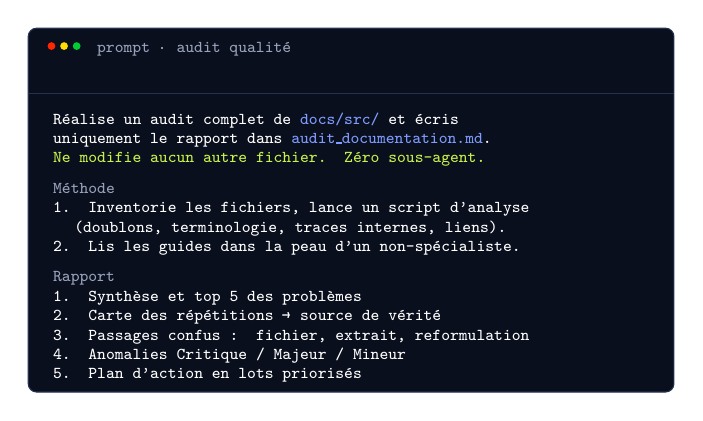
\begin{tikzpicture}[baseline=(w.north)]
      \node[fill=codebg,draw=navyline,line width=0.4pt,rounded corners=3pt,inner sep=0pt,anchor=north west] (w) at (0,0) {%
        \begin{minipage}[t][4.62cm][t]{8.2cm}
          \vspace{5pt}\hspace{7pt}%
          \tikz[baseline=-0.5ex]{\fill[red!70!orange](0,0)circle(1.4pt);\fill[yellow!80!orange](0.16,0)circle(1.4pt);\fill[green!60!teal](0.32,0)circle(1.4pt);}%
          \hspace{6pt}{\ttfamily\fontsize{5.6}{6}\selectfont\color{dmute}prompt · audit qualité}\par
          \vspace{3pt}{\color{navyline}\rule{\linewidth}{0.4pt}}\par\vspace{4pt}
          \leftskip=9pt
          \ttfamily\fontsize{5.7}{7.0}\selectfont\color{white}
          Réalise un audit complet de \kw{docs/src/} et écris\par
          uniquement le rapport dans \kw{audit\_documentation.md}.\par
          {\color{lime}Ne modifie aucun autre fichier. Zéro sous-agent.}\par
          \vspace{4pt}{\color{dmute}Méthode}\par
          1. Inventorie les fichiers, lance un script d’analyse\par
          \hspace*{1.2em}(doublons, terminologie, traces internes, liens).\par
          2. Lis les guides dans la peau d’un non-spécialiste.\par
          \vspace{4pt}{\color{dmute}Rapport}\par
          1. Synthèse et top 5 des problèmes\par
          2. Carte des répétitions → source de vérité\par
          3. Passages confus~: fichier, extrait, reformulation\par
          4. Anomalies Critique / Majeur / Mineur\par
          5. Plan d’action en lots priorisés\par
        \end{minipage}};
    \end{tikzpicture}
  \end{minipage}\hfill
  \begin{minipage}[t]{5.3cm}\vspace*{0pt}
    {\fontsize{6.8}{8.8}\selectfont\color{body}%
    \li{\textbf{\color{ink}Il sépare l’œil critique de l’écriture}~: l’agent qui relit n’a pas le droit de corriger.}
    \li{\textbf{\color{ink}Il voit ce que le build ne voit pas}~: contradictions entre chapitres, coquilles, terminologie, doublons.}
    \li{\textbf{\color{ink}Il devient la feuille de route}~: la passe 5 applique les lots en session neuve, sans ré-analyser le dépôt.}}
    \vspace{4pt}
    \noindent\chip[crit]{Critique}\,\chip[major]{Majeur}\,\chip[mute]{Mineur}
  \end{minipage}
  \par\vspace{0.2cm}
  \pull{Quelques dizaines de centimes de tokens pour une feuille de route complète.}
\end{frame}}
\note{L’audit est une session dédiée avec interdiction absolue de modifier la documentation~: l’agent ne produit qu’un rapport Markdown. Il recense les contradictions factuelles entre chapitres par gravité, les phrases tronquées et incohérences de terminologie, la carte des doublons avec la source de vérité recommandée, les passages trop denses pour un non-spécialiste, et un plan d’action en lots avec les emplacements exacts. La passe suivante, en session neuve, applique les lots dans l’ordre~: d’abord la fiabilité factuelle et la terminologie, puis la déduplication et la lisibilité. Consignes de cette passe~: localiser par titre ou grep plutôt que par vieux numéros de ligne, revérifier dans le code tout point douteux, conserver les ancres, et finir par le linter puis le build à 0 warning.}

% ===================================================================== chantier 2 · budget
{\light\kicker{01}{Chantier 2 · Le budget}
\begin{frame}{Environ 15\,€~: le budget vient de la méthode}
  \vspace{0.05cm}
  {\color{cline}\rule{\linewidth}{0.4pt}}\par\vspace{5pt}
  \tip{01}{Purger le contexte}{\code{/new} entre les phases~: on ne repaie pas des milliers de lignes de diff.}
  \tip{02}{Garder Plan → Build}{Même session du plan au build~: on ne paie pas deux fois l’exploration.}
  \tip{03}{Doser la réflexion}{Mode rapide pour le mécanique, \code{medium} pour vulgariser un moteur.}
  \tip{04}{Un seul agent}{Séquentiel et ciblé, sans sous-agents~: plus prévisible et moins cher.}
  \tip{05}{Retouches au terminal}{Un \code{grep}, un \code{git status}, trois points-virgules~: 5 secondes, 0\,€.}
  \vspace{0.1cm}
  \pull{On économise en gérant le contexte, pas en bridant les vérifications de l’agent.}
\end{frame}}
\note{Les 15 euros ne viennent pas d’une restriction aveugle. Les deux habitudes qui pèsent le plus~: repartir d’une session vierge après chaque grosse phase d’édition, et au contraire garder la même session entre le plan et son exécution. Le reste relève du bon sens~: ne pas payer un niveau de réflexion élevé pour corriger l’orthographe, ne pas multiplier les sous-agents sur une tâche bien cadrée, et faire soi-même dans le terminal ce qui prend cinq secondes. On retrouvera les outils qui vont dans le même sens à l’acte 3.}

% ===================================================================== 12 · acte 2
\actslide{02}{ACTE 2}{Mieux configurer\\OpenCode}{Des agents déclarés dans le dépôt, la bonne température et le bon modèle à chaque étape.}
  {\dchip{Anatomie d’un projet}\,\dchip{La température}\\\dchip{Les modèles}\,\dchip{Le pipeline}}
\note{Deuxième acte~: passer de ce qu’on a bricolé à une configuration propre, versionnée et partagée avec l’équipe.}

% ===================================================================== 13 · anatomie
{\dark\kicker{02}{Configurer OpenCode}
\begin{frame}{Anatomie d’un projet bien configuré}
  \vspace{0.05cm}
  \noindent\begin{minipage}[t]{4.1cm}
    \vspace*{0pt}
    \fileitem{AGENTS.md}{Conventions du projet~: le code fait foi, format RST}
    \fileitem{.opencode/agent/analyse.md}{Audit en lecture seule}
    \fileitem{.opencode/agent/writer.md}{Écriture et build}
    \fileitem{.opencode/skills/}{Skills partagés, versionnés avec le dépôt}
    \fileitem{opencode.json}{Modèles, small\_model, serveurs MCP}
  \end{minipage}\hfill
  \begin{minipage}[t]{9.3cm}
    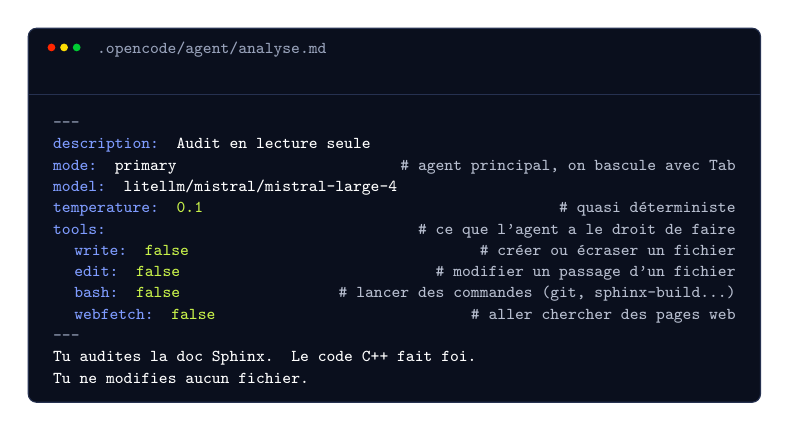
\begin{tikzpicture}[baseline=(w.north)]
      \node[fill=codebg,draw=navyline,line width=0.4pt,rounded corners=3pt,inner sep=0pt,anchor=north west] (w) at (0,0) {%
        \begin{minipage}[t][4.75cm][t]{9.3cm}
          \vspace{5pt}\hspace{7pt}%
          \tikz[baseline=-0.5ex]{\fill[red!70!orange](0,0)circle(1.4pt);\fill[yellow!80!orange](0.16,0)circle(1.4pt);\fill[green!60!teal](0.32,0)circle(1.4pt);}%
          \hspace{6pt}{\ttfamily\fontsize{5.6}{6}\selectfont\color{dmute}.opencode/agent/analyse.md}\par
          \vspace{3pt}{\color{navyline}\rule{\linewidth}{0.4pt}}\par\vspace{4pt}
          \leftskip=9pt
          \ttfamily\fontsize{6}{7.7}\selectfont\color{dmute}
          
          ---\par
          {\kw{description:} \color{white}Audit en lecture seule}\par
          {\kw{mode:} \color{white}primary}\cmt{agent principal, on bascule avec Tab}\par
          {\kw{model:} \color{white}litellm/mistral/mistral-large-4}\par
          {\kw{temperature:} \color{lime}0.1}\cmt{quasi déterministe}\par
          {\kw{tools:}}\cmt{ce que l’agent a le droit de faire}\par
          \hspace*{1.2em}{\kw{write:} \color{lime}false}\cmt{créer ou écraser un fichier}\par
          \hspace*{1.2em}{\kw{edit:} \color{lime}false}\cmt{modifier un passage d’un fichier}\par
          \hspace*{1.2em}{\kw{bash:} \color{lime}false}\cmt{lancer des commandes (git, sphinx-build…)}\par
          \hspace*{1.2em}{\kw{webfetch:} \color{lime}false}\cmt{aller chercher des pages web}\par
          ---\par
          {\color{white}Tu audites la doc Sphinx. Le code C++ fait foi.}\par
          {\color{white}Tu ne modifies aucun fichier.}\par
        \end{minipage}};
    \end{tikzpicture}
  \end{minipage}
\end{frame}}
\note{Un agent est un simple fichier markdown~: un en-tête avec modèle, température et outils autorisés, puis son prompt système. write crée ou écrase un fichier entier, edit remplace un passage précis, bash ouvre le terminal (donc git, sphinx-build, mais aussi rm). La lecture reste autorisée par défaut. Tout est versionné avec le dépôt, donc partagé avec l’équipe. À vérifier selon la version d’OpenCode installée~: le nom exact du dossier (agent ou agents) et des clés.}

% ===================================================================== 14 · température
{\light\kicker{02}{Configurer OpenCode}
\begin{frame}{La température~: régler le degré de liberté}
  \vspace{0.05cm}
  \noindent
\begin{tikzpicture}
    \def\W{13.9}
    \node[anchor=base west,inner sep=0,font=\labelfont\fontsize{5.4}{6}\selectfont,text=mute] at (0,0.42) {0 · DÉTERMINISTE};
    \node[anchor=base east,inner sep=0,font=\labelfont\fontsize{5.4}{6}\selectfont,text=mute] at (\W,0.42) {1 · CRÉATIF};
    \fill[blue] (0,0.18) rectangle (0.2*\W-0.05,0.24);
    \fill[blue!55] (0.2*\W+0.05,0.18) rectangle (0.4*\W,0.24);
    \fill[lime!70!black] (0.6*\W,0.18) rectangle (0.8*\W,0.24);
    \shade[left color=blue,right color=lime,middle color=blue!40!peri] (0,0) rectangle (\W,0.1);
  \end{tikzpicture}
  \par\vspace{0.35cm}
  \def\w{4.15cm}\def\h{1.8cm}
  \noindent\cardbox{\w}{\h}{\code{\textbf{0 – 0.2}}\par\vspace{4pt}\ctitle{Audit, extraction, vérification}\cbody{Agents analyse et vérification}}\hfill
  \cardbox{\w}{\h}{\code{\textbf{0.2 – 0.4}}\par\vspace{4pt}\ctitle{Rédaction technique, code}\cbody{Agent writer}}\hfill
  \cardbox{\w}{\h}{\code[lime!45!black]{\textbf{0.6 – 0.8}}\par\vspace{4pt}\ctitle{Reformulation, brainstorming}\cbody{Ponctuel, à la demande}}
  \par\vspace{0.8cm}
  \pull{Plus la tâche a une seule bonne réponse, plus la température doit être basse.}
\end{frame}}
\note{La température se règle par agent, dans son fichier. Pour un audit ou une vérification, on veut le même résultat à chaque fois. Pour trouver des idées de structure ou reformuler, on peut ouvrir. Ce sont des fourchettes de départ, pas des règles absolues.}

% ===================================================================== 15 · modèles
{\light\kicker{02}{Configurer OpenCode}
\begin{frame}{Quatre modèles, quatre rôles}
  \vspace{0.05cm}
  \noindent\tikz\node[card]{%
    \fontsize{6.2}{7.8}\selectfont\renewcommand{\arraystretch}{1.3}\setlength{\tabcolsep}{4pt}%
    \begin{tabular}{@{\hspace{8pt}}>{\leavevmode\ttfamily\color{blue}\raggedright\arraybackslash}p{2.45cm}>{\leavevmode\raggedright\arraybackslash}p{2.5cm}>{\leavevmode\raggedright\arraybackslash}p{6.45cm}>{\leavevmode\ttfamily\raggedleft\arraybackslash}p{0.65cm}@{\hspace{8pt}}}
      \multicolumn{1}{@{\hspace{8pt}}l}{\labelfont\fontsize{5.2}{6}\selectfont\color{mute}MODÈLE} &
      {\labelfont\fontsize{5.2}{6}\selectfont\color{mute}RÔLE} &
      {\labelfont\fontsize{5.2}{6}\selectfont\color{mute}POURQUOI} &
      \multicolumn{1}{r@{\hspace{8pt}}}{\labelfont\fontsize{5.2}{6}\selectfont\color{mute}TEMP.}\\
      \arrayrulecolor{cline}\hline
      mistral-large-4 & Planifier, auditer & {\color{body}Bon raisonnement pour écrire le plan, mais tendance connue à s’arrêter sans livrer~: à garder hors exécution} & 0.1\\ \hline
      zai-glm-5-3 & Planifier, ou exécuter les lots complexes & {\color{body}Notre REX~: efficace et moins cher. JSON d’appel d’outil parfois tronqué~: rester à température basse} & 0.2\\ \hline
      zai-glm-5-3-flash & Exécuter dès que possible, vérifier & {\color{body}Une fois le plan écrit, un modèle rapide et économique suffit pour l’appliquer, lancer le build et relire un diff} & 0.1\\ \hline
      mistral-medium-3-5 & Rédiger, traduire en français & {\color{body}Reformulations et passages en français, en appui du writer} & 0.3\\
    \end{tabular}};
  \par\vspace{0.45cm}
  \pull{Le principe~: un gros modèle planifie (Mistral Large 4 ou GLM 5.3), GLM 5.3 Flash exécute dès que la tâche le permet.}
\end{frame}}
\note{Les quatre modèles disponibles via notre LiteLLM. Le plan est l’étape qui demande le plus de raisonnement~: on la confie à un gros modèle, Mistral Large 4 ou GLM 5.3. Mistral Large 4 a été observé dans un test OpenCode qui raisonne sur un livrable sans jamais le créer~: bon pour planifier, risqué pour exécuter. Une fois le plan validé, l’exécution est plus mécanique~: GLM 5.3 Flash suffit le plus souvent, pour bien moins cher. On garde GLM 5.3 pour les lots complexes. GLM 5.x est connu pour produire parfois du JSON d’outil tronqué, d’où la température basse.}

% ===================================================================== 16 · pipeline
{\light\kicker{02}{Configurer OpenCode}
\begin{frame}{Un pipeline type, un modèle par étape}
  \vspace{0.12cm}
  \def\w{2.3cm}\def\h{3.1cm}
  \noindent\pstep{\ctag{01}}{\ctitle{Cadrer}}{\cbody{Grill Me, puis plan écrit par un gros modèle}}{\code{mistral-large-4}\par\code{ou zai-glm-5-3}}%
  \hfill\raisebox{-1.55cm}{\arr}\hfill
  \pstep[dcard]{\ctag[lime]{02}}{\ctitle[white]{Valider}}{\cbody[dmute]{Le plan, relu à la main}}{\code[lime]{Humain}}%
  \hfill\raisebox{-1.55cm}{\arr}\hfill
  \pstep{\ctag{03}}{\ctitle{Exécuter}}{\cbody{Lot par lot, un commit par lot, Handoff entre les lots}}{\code{glm-5-3-flash}\par{\fontsize{5.6}{7}\selectfont\color{body}glm-5-3 si le lot est complexe}}%
  \hfill\raisebox{-1.55cm}{\arr}\hfill
  \pstep{\ctag{04}}{\ctitle{Vérifier}}{\cbody{sphinx-build -W et relecture du diff}}{\code{un autre modèle}\par{\fontsize{5.6}{7}\selectfont\color{body}que celui qui a exécuté}}%
  \hfill\raisebox{-1.55cm}{\arr}\hfill
  \pstep[dcard]{\ctag[lime]{05}}{\ctitle[white]{Fusionner}}{\cbody[dmute]{Diff final relu, merge}}{\code[lime]{Humain}}
  \par\vspace{0.42cm}
  \pull{Un gros modèle planifie, un modèle flash exécute, et celui qui vérifie n’est jamais celui qui a produit.}
\end{frame}}
\note{Le plan, c’est là que le raisonnement compte~: Mistral Large 4 ou GLM 5.3. Une fois le plan validé, l’exécution devient mécanique~: GLM 5.3 Flash la fait dès que possible, beaucoup moins cher, et on ne repasse à GLM 5.3 que pour un lot complexe. On s’arrête, on passe le relais avec Handoff, et la vérification se fait dans une session neuve avec un modèle qui n’a pas produit le travail~: il ne se laisse pas convaincre par son propre résumé.}

% ===================================================================== 17 · acte 3
\actslide{03}{ACTE 3}{La boîte\\à outils}{Maîtriser le contexte, documenter le code, fiabiliser les livraisons de l’agent.}
  {\dchip{Le contexte}\,\dchip{La documentation}\,\dchip{La fiabilité}}
\note{Troisième acte~: les outils et skills qui répondent directement aux défauts observés pendant le chantier.}

% ===================================================================== 18 · contexte
{\light\kicker{03}{La boîte à outils}
\begin{frame}{Maîtriser le contexte, donc la consommation}
  \vspace{0.05cm}
  \noindent\begin{minipage}[t]{5.5cm}
    \vspace*{0pt}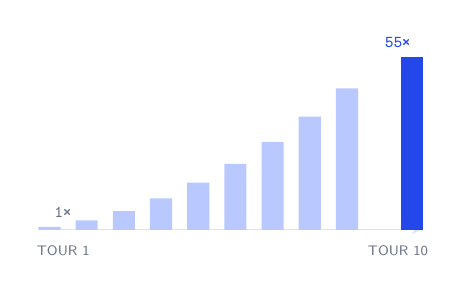
\begin{tikzpicture}
      \begin{axis}[width=6.4cm,height=3.9cm,ybar,bar width=8pt,ymin=0,ymax=58,xmin=0.4,xmax=10.6,
        axis x line=bottom,axis y line=none,xtick={1,10},xticklabels={TOUR 1,TOUR 10},
        tick style={draw=none},x axis line style={cline},
        tick label style={font=\labelfont\fontsize{5}{6}\selectfont,text=mute},
        enlargelimits=false,clip=false]
        \addplot[fill=peri!55,draw=none] coordinates {(1,1)(2,3)(3,6)(4,10)(5,15)(6,21)(7,28)(8,36)(9,45)};
        \addplot[fill=blue,draw=none] coordinates {(10,55)};
        \node[anchor=south,font=\ttfamily\fontsize{6.4}{7}\selectfont\bfseries,text=blue] at (axis cs:10,55) {55×};
        \node[anchor=south,font=\ttfamily\fontsize{5.6}{7}\selectfont,text=mute] at (axis cs:1,1) {1×};
      \end{axis}
    \end{tikzpicture}\par\vspace{2pt}
    {\raggedright\fontsize{5.8}{7.4}\selectfont\color{body}Coût cumulé si chaque tour ajoute autant de texte (illustratif)~: 10 tours ≈ 55 fois le premier.}
  \end{minipage}\hfill
  \begin{minipage}[t]{7.9cm}
    \vspace*{0pt}{\fontsize{8}{10}\selectfont\bfseries Les leviers, du moins cher au plus outillé}\par\vspace{6pt}
    \lever{01}{Une session par tâche}{Gratuit et immédiat.}
    \lever{02}{Handoff}{Repartir d’un résumé structuré, pas d’une session fleuve.}
    \lever{03}{RTK}{Compresse la sortie shell~; \code{rtk gain} chiffre le gain.}
    \lever{04}{Serena}{Interroge un symbole au lieu de lire des fichiers entiers.}
  \end{minipage}
\end{frame}}
\note{Pourquoi la conso explose~: à chaque tour, tout l’historique est renvoyé au modèle. Si chaque tour ajoute la même quantité de texte, dix tours coûtent environ 55 fois le premier. C’est un modèle simplifié, pas une mesure. RTK s’installe dans OpenCode avec rtk init -g --opencode. Serena est un serveur MCP local basé sur les language servers.}

% ===================================================================== 19 · documenter
{\light\kicker{03}{La boîte à outils}
\begin{frame}{Documenter et comprendre le code}
  \vspace{0.12cm}
  \def\w{4.15cm}\def\h{3.5cm}
  \noindent\cardbox[bcard]{\w}{\h}{\tagbox{La vedette}\ctitle{Graphify}\cbody{Cartographie le projet (code, docs, PDF, images) en un graphe de connaissances qu’on interroge au lieu de faire des grep.}\cardfoot{Code analysé en local (Tree-sitter). Docs et images passent par le LLM.}}\hfill
  \cardbox{\w}{\h}{\tagbox{Wiki privé}\ctitle{Local DeepWiki MCP}\cbody{Génère une doc façon wiki pour un dépôt privé, avec questions-réponses par RAG.}\cardfoot{100\,\% hors ligne possible~: Ollama et sentence-transformers.}}\hfill
  \cardbox{\w}{\h}{\tagbox{Relecture}\ctitle{stop-slop}\cbody{Repère et réécrit les tics d’écriture de l’IA dans les README, commits et docs.}\cardfoot{Skill markdown local, sans service externe.}}
  \par\vspace{0.42cm}
  \pull{Démo proposée~: \texttt{/graphify} sur LP-ShiftPlanner, puis une question d’architecture.}
\end{frame}}
\note{Graphify installe aussi un rappel dans AGENTS.md et un plugin OpenCode pour que l’agent consulte le graphe avant de fouiller les fichiers~: il fait donc aussi économiser des tokens. stop-slop sert pour les livrables clients qui ne doivent pas sentir l’IA.}

% ===================================================================== 20 · coder
{\light\kicker{03}{La boîte à outils}
\begin{frame}{Coder sereinement~: cadrer, vérifier, passer le relais}
  \vspace{0.12cm}
  \def\w{4.15cm}\def\h{3.5cm}
  \noindent\cardbox{\w}{\h}{\ctitle{Superpowers}\cbody{Planification, sous-agents, TDD, débogage. Son skill phare force la vérification avant de conclure~:}\vspace{3pt}\code{verification-before-completion}\cardfoot[orange]{Télémétrie active par défaut~: à désactiver.}}\hfill
  \cardbox{\w}{\h}{\ctitle{Grill Me}\cbody{Vous interroge sur chaque branche du plan avant la première ligne de code, avec une réponse recommandée.}\cardfoot{Répond à~: plans flous, mauvaises surprises.}}\hfill
  \cardbox{\w}{\h}{\ctitle{Handoff}\cbody{Condense la session dans un markdown structuré, repris par une nouvelle session ou un autre agent.}\cardfoot{Répond à~: contexte qui gonfle, coût qui grimpe.}}
  \par\vspace{0.42cm}
  \pull{Superpowers répond directement au défaut observé chez Mistral~: s’arrêter sans livrer.}
\end{frame}}
\note{Trois skills de méthode. Grill Me formalise ce qu’on a fait à la main dans la passe 1. Handoff permet d’arrêter GLM quand le gros est fait et de lancer la vérification dans une session propre.}

% ===================================================================== 21 · checklist
{\limeslide\kicker{04}{À retenir}
\begin{frame}{La checklist}
  \vspace{0.05cm}
  \noindent\begin{minipage}[t]{6.65cm}
    \ck{Un plan écrit avant de lancer}
    \ck{Le bon modèle pour la bonne tâche}
    \ck{Un agent par rôle, des droits minimaux}
    \ck{La bonne température pour la tâche}
    \ck{Plusieurs passes sur les parties clés}
    {\color{ink!25}\rule{\linewidth}{0.4pt}}
  \end{minipage}\hfill
  \begin{minipage}[t]{6.65cm}
    \ck{Un critère de validation automatique}
    \ck{Dire ce qu’il ne doit pas toucher}
    \ck{Handoff plutôt que sessions fleuves}
    \ck{Un commit par étape}
    \ck{Un audit en lecture seule avant de corriger}
    {\color{ink!25}\rule{\linewidth}{0.4pt}}
  \end{minipage}
\end{frame}}
\note{La slide à photographier. Dix réflexes, tous issus des deux chantiers.}

\end{document}
